% !TEX TS-program = xelatex
% !TEX encoding = UTF-8 Unicode
% !Mode:: "TeX:UTF-8"

\documentclass{resume}
\usepackage{graphicx}
\usepackage{tabu}
\usepackage{multirow}
\usepackage{progressbar}
\usepackage{zh_CN-Adobefonts_external} % Simplified Chinese Support using external fonts (./fonts/zh_CN-Adobe/)
% \usepackage{NotoSansSC_external}
% \usepackage{NotoSerifCJKsc_external}
% \usepackage{zh_CN-Adobefonts_internal} % Simplified Chinese Support using system fonts
\usepackage{linespacing_fix} % disable extra space before next section
\usepackage{cite}
\usepackage{fontspec}

\usepackage{hyperref}
\hypersetup{
    colorlinks=true,
    linkcolor=blue,
    filecolor=blue,      
    urlcolor=blue,
    citecolor=cyan,
}

\begin{document}
\pagenumbering{gobble} % suppress displaying page number

\Large{
  \begin{tabu}{ c l l }
   \multirow{4}{1in}{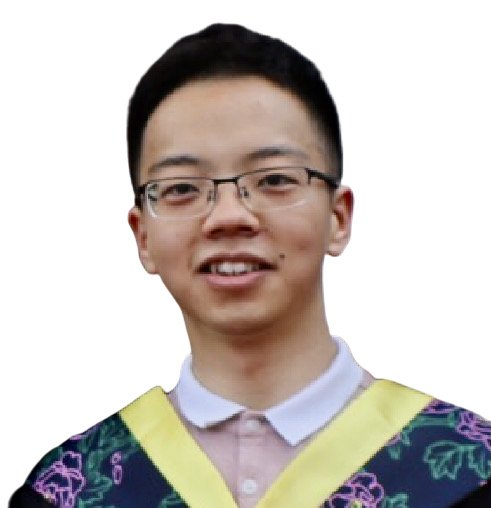
\includegraphics[width=0.95in]{me.jpeg}} & \scshape{Xueyao Zhang(张雪遥)} &  \\
    & \email{zhangxueyao19s@ict.ac.cn} & \phone{~~(+86) 152-0390-0168} \\
    % & \phone{(+86) 152-0390-0168} &  \\
    & \faWechat{ xueyao\_98} & \github[~~github.com/RMSnow]{https://github.com/RMSnow} \\
    & \faHome{\href{https://www.zhangxueyao.com}{~~zhangxueyao.com}}
    & \faGraduationCap {\href{https://scholar.google.com/citations?user=lf1udBcAAAAJ&hl=en}{~~Google Scholar}} 
  \end{tabu}
}

\section{Education}
\datedsubsection{\textbf{Institute of Computing Technology, Chinese Academy of Sciences}}{Sept. 2019 -- Jun. 2022}
{
  \small 
  % 前瞻实验室,研究方向:虚假新闻检测、事实核查,导师:\href{http://www.ict.cas.cn/sourcedb_2018_ict_cas/cn/jssrck/201011/t20101123_3028158.html}{曹娟}研究员;GPA:3.79 / 4.00.
\begin{itemize}
  \item Master candidate in Computer Application Technology (being recommended for admission)
  \item Areas of Study: Fake News Detection
  \item Advisor: Professor Juan Cao
  \item GPA: 3.79 / 4.00
\end{itemize}
}

\datedsubsection{\textbf{School of Computer Science, Wuhan University}}{Sept. 2015 -- Jun. 2019}
{
  \small 
  % GPA:3.84 / 4.00,专业排名:4 / 246,英语六级:522.
\begin{itemize}
  \item B.Eng in Software Engineering
  \item GPA: 3.84 / 4.00, Ranking: 4 / 246 (Top 1.6\%)
\end{itemize}
}


\section{Publications}
\textbf{\large \framebox[1.2\width]{Fake News Detection}}

\datedsubsection{\textbf{1.} \quad \textit{\textbf{Mining Dual Emotion for Fake News Detection} (Long Paper; Oral; First-authored)}}{}
{\small \role{\textbf{\underline{Xueyao Zhang}}, Juan Cao, Xirong Li, Qiang Sheng, Lei Zhong, Kai Shu.}{Proceedings of the 30th Web Conference \textbf{(WWW 2021)}\quad \href{https://www.zhangxueyao.com/data/www2021-dual-emotion-paper.pdf}{[PDF]} \href{https://github.com/RMSnow/WWW2021}{[Code]} \href{https://www.zhangxueyao.com/data/www2021-dual-emotion-slides.pdf}{[Slides]} \href{https://www.zhangxueyao.com/data/www2021-dual-emotion-video.mp4}{[Video]} \href{https://www.bilibili.com/video/BV13o4y1m7c3}{[Chinese Video]}
}
\small
\textit{TL;DR}: We leverage both publisher emotion and social emotion for fake news detection.

\datedsubsection{\textbf{2.} \quad \textit{\textbf{Integrating Pattern- and Fact-based Fake News Detection via Model Preference Learning} (Long Paper; Oral; Co-first-authored)}}{}
{\small \role{Qiang Sheng*, \textbf{\underline{Xueyao Zhang}}*, Juan Cao, Lei Zhong. (*: Equal Contribution)}{Proceedings of the 30th ACM International Conference on Information and Knowledge Management \textbf{(CIKM 2021)}\quad \href{https://dl.acm.org/doi/10.1145/3459637.3482440}{[PDF]} \href{https://www.zhangxueyao.com/data/cikm2021-PrefFEND-poster.pdf}{[Poster]} \href{https://github.com/ICTMCG/Pref-FEND}{[Code]} \href{https://zhuanlan.zhihu.com/p/414464291}{[Chinese Blog]}}
}
\small
\textit{TL;DR}: We propose a graph-based model preference learning framework to separately handle the pattern and fact indicators in fake news detection.

\datedsubsection{\textbf{3.} \quad \textit{\textbf{Article Reranking by Memory-enhanced Key Sentence Matching for Detecting Previously Fact-checked Claims} (Long Paper; Poster; Second-student-authored)}}{}
{\small \role{Qiang Sheng, Juan Cao, \textbf{\underline{Xueyao Zhang}}, Xirong Li, Lei Zhong.}{Proceedings of the Joint Conference of the 59th Annual Meeting of the Association for Computational Linguistics \textbf{(ACL 2021)}\quad \href{https://aclanthology.org/2021.acl-long.425.pdf}{[PDF]} \href{https://www.zhangxueyao.com/data/acl2021-MTM-poster.pdf}{[Poster]} \href{https://github.com/ICTMCG/MTM}{[Code]} \href{https://zhuanlan.zhihu.com/p/393615707}{[Chinese Blog]}}
\small
\textit{TL;DR:} We detect previously fact-checked claims by matching them against the key sentences in fact-checking articles.

\datedsubsection{\textbf{4.} \quad \textit{\textbf{Zoom Out and Observe: News Environment Perception for Fake News Detection} (Long Paper; Second-student-authored)}}{}
{\small \role{Qiang Sheng, Juan Cao, \textbf{\underline{Xueyao Zhang}}, Rundong Li, Danding Wang, Yongchun Zhu.}{\textbf{(Under Review)}}
\small
\textit{TL;DR}: We leverage the external news environment where a news post is created and disseminated for detecting fake news.

\textbf{\\ \large \framebox[1.2\width]{Music Generation}}
\datedsubsection{\textbf{1.} \quad \textit{\textbf{Structure-Enhanced Pop Music Generation via Harmony-Aware Learning} (Long Paper; First-authored)}}{}
{\small \role{\textbf{\underline{Xueyao Zhang}}, Jinchao Zhang, Yao Qiu, Li Wang, Jie Zhou.}{\textbf{(Under Review)}\quad \href{https://arxiv.org/pdf/2109.06441.pdf}{[Preprint]}}
}
\small
\textit{TL;DR}: We propose to learn harmony for generating form- and texture- enhanced pop music.

\section{Academic Services}
\datedsubsection{\textbf{Reviewer / PC Member}}{}
\begin{itemize}
  \item EMNLP 2021
  \item ACM CSCW 2021
  \item Information Processing and Management
\end{itemize}

\section{Internships}
\datedsubsection{\faWechat{} \textbf{Wechat, Tencent}}{Apr. 2021 -- Present}
{\small \role{Research Intern, Pattern Recognition Center of Wechat AI, Beijing, China
}{}
}
% \small
\begin{itemize}
  \item Music Generation Research \& Development.
  \item Supply the support for the knowledge of music, including music theory. 
  \item In May 2021, I gave a talk on music, \href{https://www.zhangxueyao.com/data/wcpr-pop-music.pdf}{\underline{How to create a pop song?}}
\end{itemize}

\section{Teaching Experiences}
\datedsubsection{\textbf{Teaching Assistant, Wuhan University}}{2017 Fall}
\small
Object-Oriented Programming (JAVA), School of Computer Science

\section{Honors and Awards}
\begin{itemize}
  \item National Graduate Scholarship, Ministry of Education of China (Top1\%, 2021)
  \item National Undergraduate Scholarship, Ministry of Education of China (Top1\%, 2016)
  \item Third place at Campus Singer Competition, University of Chinese Academy of Sciences(Top3, 2020)
  \item Excellent Bachelor Thesis, Wuhan University (Top5\%, 2019)
  \item First price in Chinese High School Mathematics League (Top50 in Henan Province, 2014)
  \item Merit Student, University of Chinese Academy of Sciences (2019; 2020)
  \item Merit Student and Outstanding Student Leaders, Wuhan University (2016; 2017; 2018)
\end{itemize}

\section{Musical Abilities}
\begin{itemize}
  \item Familiar with the basic music theory.
  \item Familiar with and capable of distinguishing the common musical genres.
  \item Proficient in playing pop keyboard.
  \item Proficient in pop singing, and familiar with Bel canto.
\end{itemize}

\section{Programming Skills}
\begin{itemize}
  \item Programming Languages: proficient in Python, familiar with Java, and know about C++.
  \item Deep Learning Frameworks: proficient in PyTorch and Keras.
\end{itemize}

\end{document}
